\documentclass{article}

\usepackage{fontspec}
\usepackage{xeCJK}
\setmainfont{Times New Roman}
\setCJKmainfont{Hiragino Mincho ProN}
\setCJKsansfont{Hiragino Kaku Gothic ProN}
\setCJKmonofont{Hiragino Kaku Gothic ProN}
\XeTeXlinebreaklocale "ja"
\XeTeXlinebreakskip = 0pt plus 1pt
\renewcommand{\baselinestretch}{1.3}
\usepackage{geometry}
\geometry{verbose,tmargin=2cm,bmargin=2cm,lmargin=2.5cm,rmargin=2.5cm}
\usepackage{amsmath}
\usepackage{amsfonts}
\usepackage{bm}
\usepackage{graphicx}
\usepackage{authblk}
\usepackage{url}
% for hyperref
\usepackage[bookmarkstype=toc, colorlinks=false, pdfborder={0 0 0}, bookmarks=true, bookmarksnumbered=true]{hyperref}

\renewcommand{\figurename}{図}
\renewcommand{\tablename}{表}


\begin{document}

\title{宇宙機の姿勢決定}

\author[1]{yasuhiro yoshimura}
\affil[1]{Kyushu University, y.yoshimura.a64@m.kyushu-u.ac.jp}

\maketitle
% \tableofcontents


\section{目的}
燃料補給,修理,デブリ除去といった宇宙機の軌道上サービスミッション(On-Orbit Servicing, OOS)では,自身の状態だけでなく,ターゲットの相対軌道・姿勢を決定することが求められる.
本実験では,カメラで撮像されたターゲットの画像を用いた相対姿勢決定を扱う.

\section{基礎}
\subsection{軌道上サービスミッション(On-Orbit Servicing, OOS)}
燃料補給,修理,デブリ除去といった軌道上の物体に対する近接運用を軌道上サービスと呼ぶ.OOSは一般に1)アプローチ,2)観測,3)サービス,4)軌道遷移の4つのフェイズからなる.本実験は2)観測フェイズにおける相対姿勢推定を想定する.
光学カメラは低コストであり,遠距離から近距離まで対応可能であることから相対状態推定に用いられる.
光学カメラを用いた姿勢推定の古典的な手法に特徴点を用いたものがあるが,軌道上は地球アルベド以外の反射光がないため,姿勢による陰がはっきりと現れ(例えばAstroscale社による図~\ref{fig:h2a}),マッチングが困難になることがある.また光学条件が軌道周回によって変化することも難しさのひとつである.
\begin{figure}[tb]
\centering
\includegraphics[width=8cm]{./figs/astroscaleH2A.png}
\caption{軌道上のH2A上段 (c)Astroscale}
\label{fig:h2a}
\end{figure}

\subsection{姿勢}\label{sec:attitude}
宇宙機の``姿勢''を定義する.ここでは姿勢を``2つの座標系を結ぶ回転''として定義する.
例えば,空間に固定された慣性座標系($i$系)と宇宙機に固定された機体固定座標系($b$系)を設定し,$i$系を回転させて$b$系に一致させることを考える(Fig.~\ref{fig:i2b}).その回転を適当なパラメータ($\phi,\theta,\psi$など)で定量的に表したものが宇宙機の``姿勢''(厳密には$i$系に対する$b$系の姿勢)である.

座標系は何でも良く,RSW座標系を回転させて,$b$系に一致させる場合,その回転(つまり姿勢)はRSW座標系に対する宇宙機($b$系)の姿勢を意味する.
$b$系を回転させてRSW座標系へ一致させる回転は意味が異なり,その回転の場合は$b$系に対するRSW系の姿勢になってしまう.
そのため,どの座標系に対する姿勢なのか,を意識することが大事である.
また,基本的に宇宙機の姿勢を扱う場合は,ある基準座標系(慣性系やRSW系)に対する宇宙機の姿勢を考えるため,基準座標系を回転させて$b$系に一致させる回転を宇宙機の姿勢とする.
(つまり,$b$系を回転させて,基準座標系へ一致させる回転を宇宙機の姿勢とはしない.)
\begin{figure}[tb]
\centering
\includegraphics[width=7cm]{./figs/i2b.pdf}
\caption{座標系の回転}
\label{fig:i2b}
\end{figure}

\subsection{オイラー角}
オイラー角は直観的理解が容易で,頻繁に使われる姿勢表現である.
各座標軸($x,y,z$)周りの連続する3回転によって表現される.
回転角$\beta$に対する$x,y,z$軸の周りの回転行列はそれぞれ
\begin{align}
R_{x}(\beta)&=\begin{bmatrix}
1  &  0  &  0\\
 0  &  \cos\beta\   &  \sin\beta\\
 0  &  -\sin\beta\   &  \cos\beta
\end{bmatrix} \\
R_{y}(\beta) &= \begin{bmatrix}
\cos\beta & 0 & -\sin\beta\\
0 & 1 & 0\\
\sin\beta & 0 & \cos\beta
\end{bmatrix}\\
R_{z}(\beta)&=\begin{bmatrix}
\cos\beta & \sin\beta & 0\\
-\sin\beta & \cos\beta & 0\\
0 & 0 & 1
\end{bmatrix}
\end{align}
となる.
この基本的な回転行列を組み合わせることで全てのオイラー角の回転行列が計算される.

例えばZYXオイラー角を用いた$i$系から$b$系への回転行列$R_{b/i}$は
\begin{align}
R_{b/i} & =R_{x}(\psi)R_{y}(\theta)R_{z}(\phi)\\
&= \left[\begin{array}{ccc}
\cos\theta\cos\phi & \cos\theta\sin\phi & -\sin\theta\\
\sin\theta\sin\psi\cos\phi-\cos\psi\sin\phi & \sin\theta\sin\psi\sin\phi+\cos\psi\cos\phi & \cos\theta\sin\psi\\
\sin\theta\cos\psi\cos\phi+\sin\psi\sin\phi & \sin\theta\cos\psi\sin\phi-\sin\psi\cos\phi & \cos\theta\cos\psi
\end{array}\right]
\end{align}
となる.
他のオイラー角(XYZなど)の回転行列を求める場合は,各軸回りの回転行列の順序を変えるだけで良い(e.g.,XYZオイラー角は$R_{b/i}=R_{z}(\psi)R_{y}(\theta)R_{x}(\phi)$である).

\subsection{固有空間法}
本実験では姿勢決定に固有空間法を用いる~\cite{10.1299/jsmermd.2013._2p1-m08_1,10.2322/jjsass.64.253}.固有空間法はターゲットの様々な姿勢の画像を学習データとし,その共分散から固有空間を生成する.
そして,推定したい姿勢の画像をその固有空間に射影することで姿勢決定を行う.

学習データの画素数を$M$,学習データ数を$N$とする.画像を$M$次元ベクトルとして,学習データ行列を
\begin{align}
X = [\bm{x}_{1},\bm{x}_{2},\cdots,\bm{x}_{N}] \in \mathbb{R}^{M\times N}
\end{align}
と表すことができる.
平均ベクトル
\begin{align}
\bm{c}  = \frac{1}{N}\sum_{i=1}^{N} \bm{x}_{i}
\end{align}
を用いて学習データの平均ゼロ化を次式で行う.
\begin{align}
\bar{X} = [\bm{x}_{1}-\bm{c},\cdots, \bm{x}_{N}-\bm{c}]
\end{align}
共分散
\begin{align}
Q = \frac{1}{N}\bar{X}\bar{X}^{T}
\end{align}
を計算し,その固有ベクトルを$\bm{e}_{i}$ (i=1,\dots, N)とする.
固有値の大きい上位$k$個の用いて固有空間を形成する.
この固有空間に対して,例えば$i$番目の画像を
\begin{align}
\hat{\bm{x}}_{i} = [\bm{e}_{1},\bm{e}_{2},\cdots, \bm{e}_{k}]^{T} (\bm{x}_{i}- \bm{c})
\end{align}
として固有間に射影する.このベクトル$\hat{\bm{x}}_{i}$は$k$次元ベクトルであり,$M$次元の情報が$k$次元に圧縮されている.次元$k$の決め方は寄与率とその累積を用いることができる.寄与率は
\begin{align}
s_{j} = \frac{\lambda_{j}}{\sum_{i=1}^{M}\lambda_{i}}
\end{align}
と定義され,$j$番目の学習データが画像をどの程度表現できるかを示す.ここで$\lambda_{i}$は$i$番目の固有値である.
累積寄与率$t_{j}$は上位$j$番目までの固有空間の寄与率の合計,つまり
\begin{align}
t_{j} = \sum_{i=1}^{j}s_{i}
\end{align}
と計算される.

姿勢推定したいターゲットの画像を$y\in \mathbb{R}^{M}$とする.同様に,平均ゼロ化し,固有空間へ射影する.
\begin{align}
\hat{\bm{y}} = [\bm{e}_{1},\bm{e}_{2},\cdots, \bm{e}_{k}]^{T} (\bm{y}- \bm{c})
\end{align}
(素朴には)この$\hat{\bm{y}}$と固有空間における学習データ$\hat{\bm{x}}_{i}  (i=1,\dots, N)$とのユークリッド距離が最小になる姿勢を推定姿勢とする.


\section{構成・仕様}
実験装置は図~\ref{fig:config}のように構成される.
ロボットアーム先端に宇宙機モデルを設置し,アームにより回転させることができる.
平行光源を任意の方向からモデルへ照射し,リニアレール上のカメラからターゲットを撮像する(撮像例:図~\ref{fig:testShot}).
測定時は外乱光を抑制するために,暗幕を用いる.
ロボットアームと平行光の仕様は表~\ref{tab:armLight}のとおりである.

\begin{figure}[h]
\centering
\includegraphics{./figs/config.pdf}
\caption{装置構成}
\label{fig:config}
\end{figure}

\begin{figure}[tb]
\centering
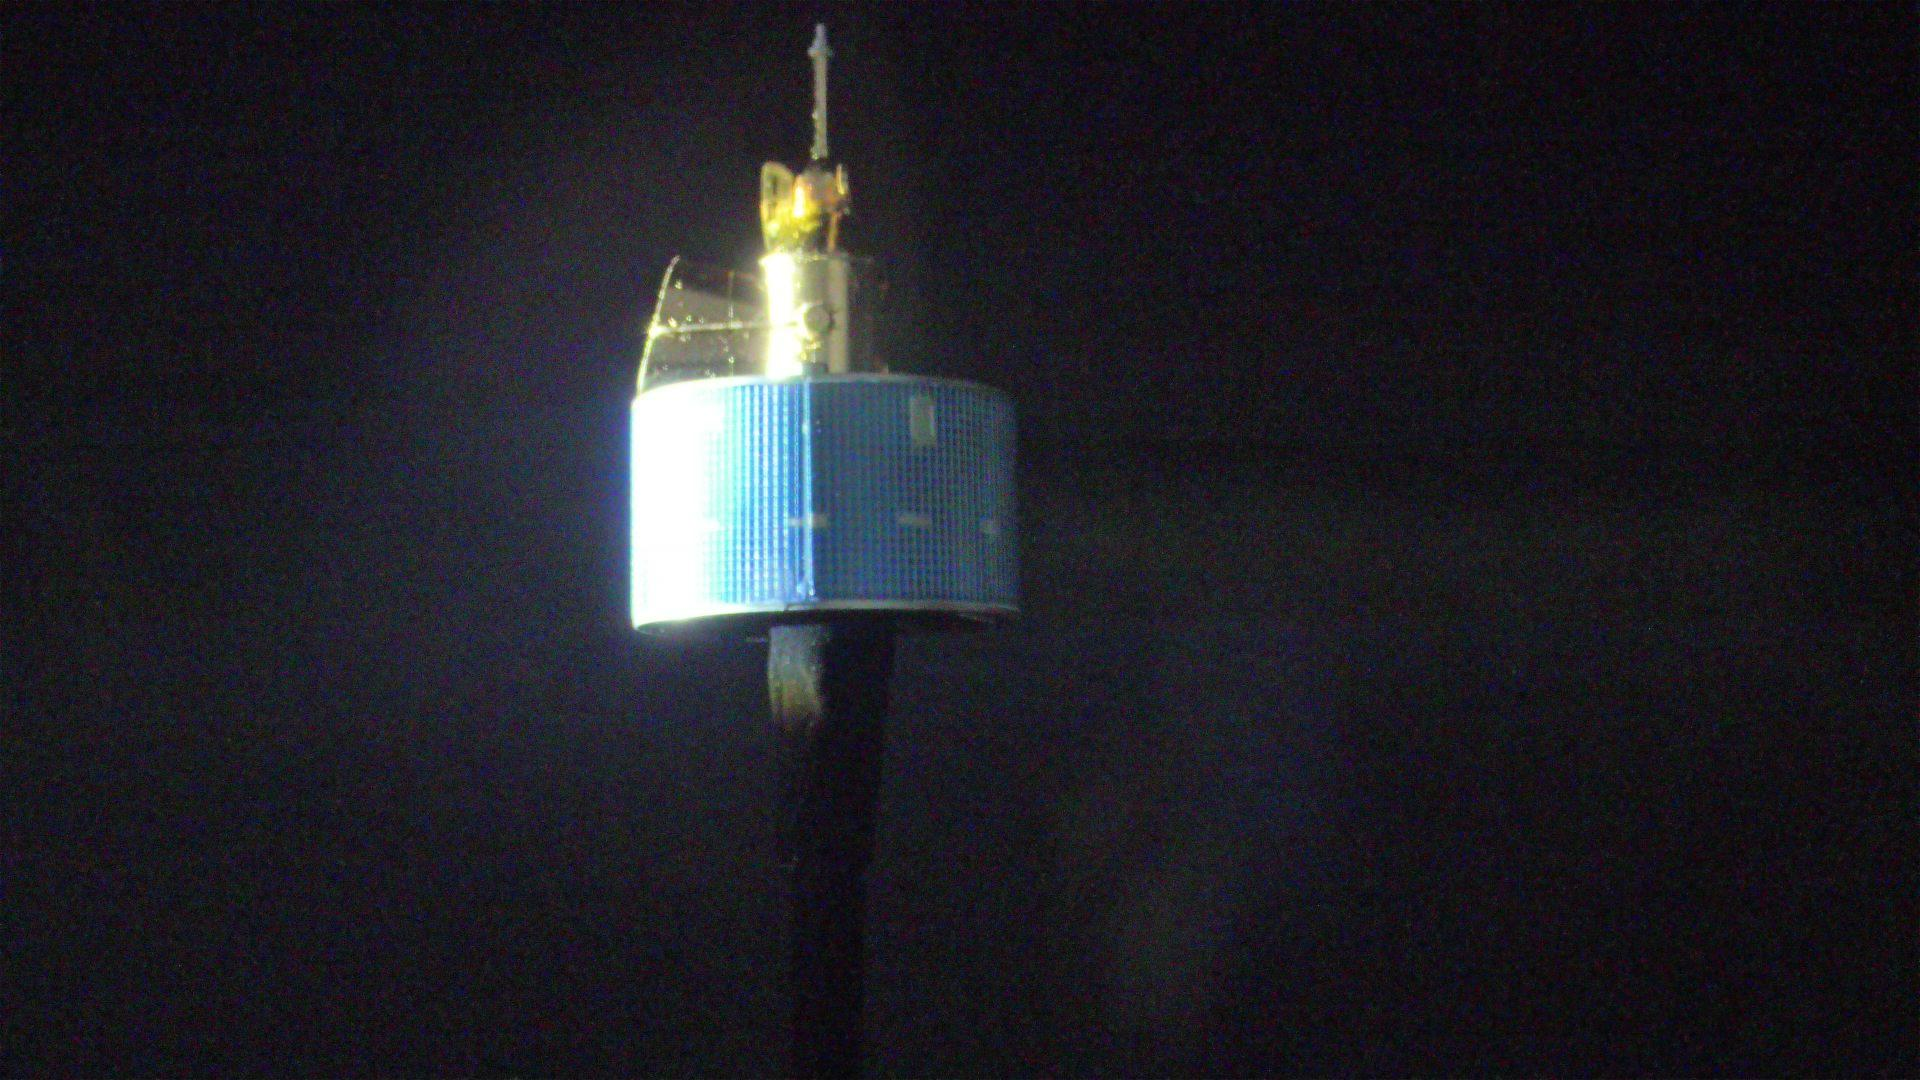
\includegraphics[width=7cm]{./figs/testShot.jpeg}
\caption{撮像例}
\label{fig:testShot}
\end{figure}

\begin{table}[htb]
\begin{center}
\caption{ロボットアームと光源の諸元} \label{tab:armLight}
\begin{tabular}{lc|lc} 
\hline \hline
製品 & UFACTORY LITE 6 & 製品 & ホロライト\\
自由度 & 6  & 電力 & 3 W\\
動作領域図 & ~\ref{fig:arm}参照 &配光特性(広がり角) & $0.48-15$ deg \\ 
\hline \hline
\end{tabular}
\end{center}
\end{table}

\begin{figure}[tb]
\centering
\includegraphics[width=6cm]{./figs/robotArm.pdf}
\caption{ロボットアーム動作範囲}
\label{fig:arm}
\end{figure}

\section{手順}
本実験の目的は,1)学習・テストデータの取得,2)PythonやMATLABを用いた学習データによる固有空間構築,3)構築した固有空間よる姿勢決定である.
ただし問題の簡単化のため,シングルスピン運動のみを扱う.
姿勢決定精度への影響を及ぼす変数として,学習データ数・種類,固有空間次元$k$,画像解像度,光学条件,ターゲット形状等がありうる.

\subsection{予備検討}
\begin{enumerate}
\item ターゲット物体をスピン衛星,box-wing衛星,円柱ボディから選定.
\item 学習データの数と種類を検討.(どの姿勢角で撮像するか,CGモデルも使うか)
\item 光学条件(光源とカメラの位置・向き)を決定.
\end{enumerate}

\subsection{データ取得}
\begin{enumerate}
\item 光源の位置・姿勢とロボットアームの位置・姿勢を調整する.
\item ターゲット物体を複数角度で撮影し,学習画像データセットを取得.
\item 姿勢決定アルゴリズムを適用するテストデータセット(シングルスピン)を取得(学習データの一部をテストデータとして使用しても良い).
\end{enumerate}

\subsection{姿勢決定}
\begin{enumerate}
\item 学習データ画像をグレースケール化・リサイズなどの前処理を施す.
\item 学習データから主成分分析(固有空間法)を実施し,固有空間を構築.(他の姿勢決定を用いても良い)
\item 推定した姿勢を実際の姿勢(ロボットアームの角度を真値とする)を比較し,考察.
\end{enumerate}

考察の例:
\begin{itemize}
\item 固有空間の次元数が推定精度に与える影響
\item 画像サイズや解像度と推定精度の関係
\item 光源の向き・明るさなど光学条件が推定に与える影響
\item 推定誤差が生じる原因とその対処法
\end{itemize}

% \subsection{操作手順}
% \begin{enumerate}
%     \item ロボットアームを図~\ref{fig:armConfig}にしたがって設定し,initial positionとして保存する.
%     \item ロボットアームのpayloadをsunsensorにし,attitude stepを10 degに設定して保存する.
%     \item ロボットアーム先端に太陽センサを取り付ける.
%     \item 平行光のボリュームを落とし,フォーカスと照射位置が太陽センサ中央になるように設置する.設置後にボリュームを最大にする.
%     \underline{平行光やその反射を直視しないように注意する.}
%     \item 太陽センサにつながっているarduinoをmacに接続し,MATLABでデータ読み取りプログラムを実行し,動作を確認する.
%     \item センサをロボットアーム座標系$z_{r}$,$y_{r}$軸周りにそれぞれ0 degを中心とした10 deg刻みで$\pm 60~{\rm deg}$回転させ,データを取得する.図~\ref{fig:frame}に座標系を示す.太陽センサの座標系は破線で示される.
%     \item 最後に未知の角度に対するデータを2ケース取得する.
% \end{enumerate}

\vspace{\baselineskip}

\section{レポート}
グループでひとつのレポートを作成する.
原理,手順,仕様は省略可.目的,データ処理・姿勢決定方法,結果と考察,結論等を端的に述べる.
データはDropbox(下記URL)からダウンロードできる.

提出期限・方法
\begin{itemize}
    \item 提出期限: 実施日翌週の月曜日20時
    \item 提出先: Moodle
    \item ファイルフォーマット: pdf    
\end{itemize}

\section*{Appendix}
MATLABのプログラムと取得したデータはGitHubにuploadしている.
\begin{itemize}
    \item \texttt{changeNames.m}は指定したディレクトリの\texttt{jpeg}ファイルを連番ファイル名に変更する.(実験で得られる画像ファイル名はタイムスタンプ.)
    \item \texttt{mainEigenSpace.mlx}は学習データとテストデータを読み込み,固有空間法により姿勢決定するものである.
星印は変更が必要な箇所(パラメータ)を意味する.
\end{itemize}




\bibliographystyle{plain}
\bibliography{yoshimura}

\end{document}